\section{Laboratory work implementation}

\subsection{Tasks and Points}

- Fiecare din membrii echipei va lucra pe propriul branch in git, iar una din persoane va avea grija sa faca merge cu master; \\
\indent 
- Proiectul se poate afla doar in repozitoriul unui membru al echipei; \\
\indent 
- Dezvoltarea unei aplicatii: Mobile;

\subsection{Analiza lucrarii de laborator}
\selectlanguage{russian}
В ходе данной лабораторной работы было разработано приложение на подобии записной книжки.Моя часть лаборатоной работы состояла в реализации пользователского интерфейса и адартера для использования данных с БД.\\
\indent
Для выбора изобрадения использовалась стандартная галереяю.Для отображения списка использовали RecycleView. \\
\indent
Для улучшения производительности использовали новые потоки, чтобы не загружать основной UI поток.Также для улучшения производительности использовался кэш,для быстрого доступа к изображениям  




\subsection{Imagini}

\begin{figure}[h]
	\center{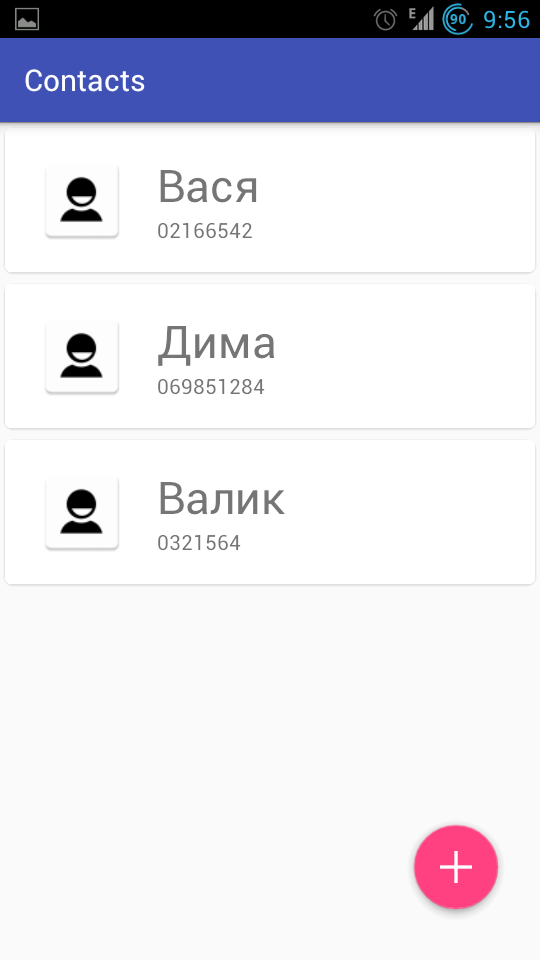
\includegraphics[width=1\linewidth]{images/1.png}}
	\caption{Заглавное меню}
	\label{ris:image}
\end{figure}
\hfill
\begin{figure}[h]
	\center{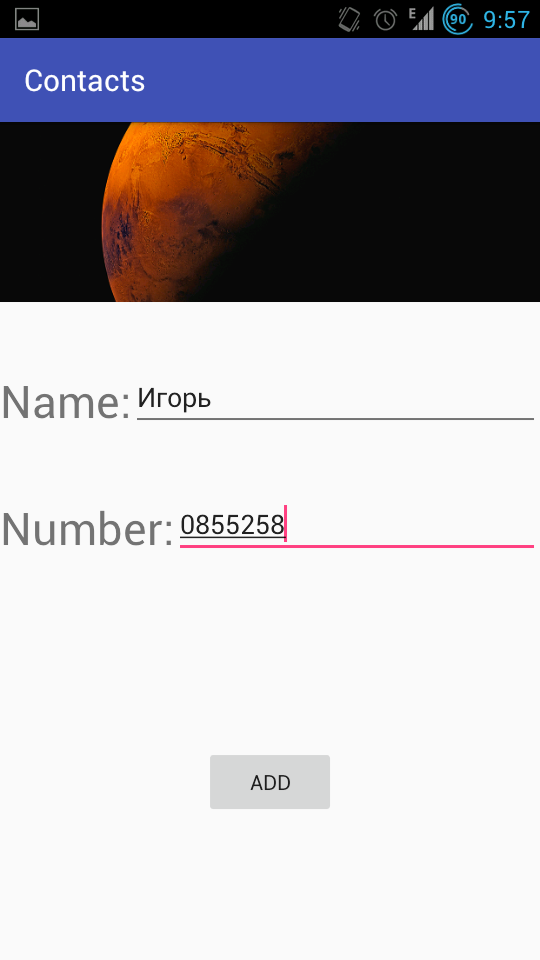
\includegraphics[width=1\linewidth]{images/2.png}}
	\caption{Добавление контакта в БД}
	\label{ris:image}
\end{figure}
\hfill
\begin{figure}[h]
	\center{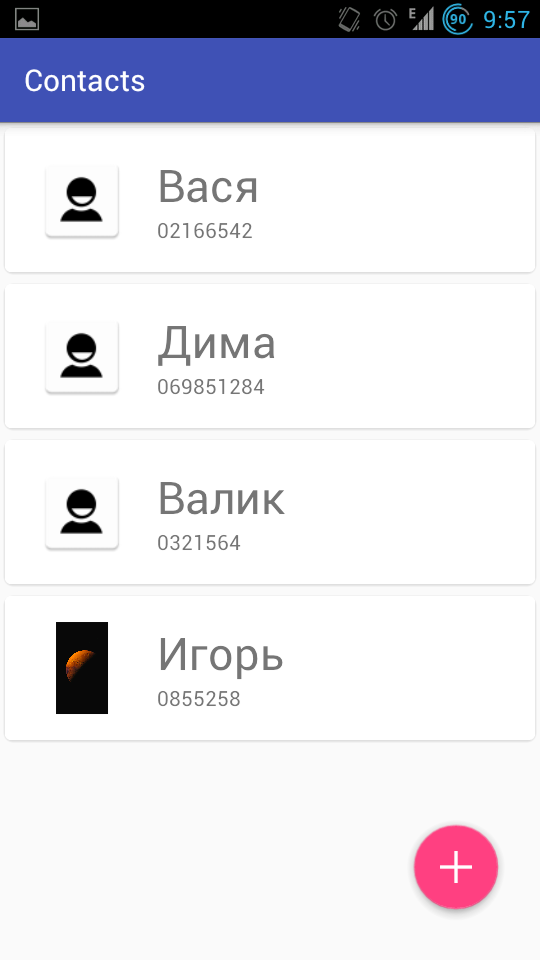
\includegraphics[width=1\linewidth]{images/3.png}}
	\caption{Результат добавления пользователя}
	\label{ris:image}
\end{figure}
\hfill
\begin{figure}[h]
	\center{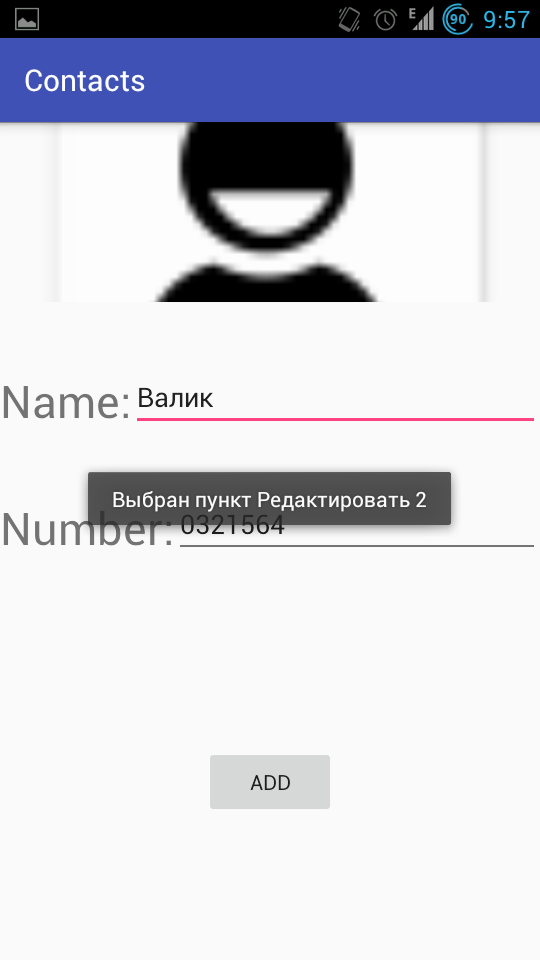
\includegraphics[width=1\linewidth]{images/4.png}}
	\caption{Редактирования данных пользователя}
	\label{ris:image}
\end{figure}

\clearpage